\chapter{Experimentation}
In this chapter we experiment with the MultiChain community implemented within Tribler.
We test if MultiChain is correctly implemented according to the design.
MultiChain is experimented with to test if it can correctly create a chain tracking a download.
Next, MultiChain is experimented with tracking anonymous downloads.
Finally, MultiChain is experimented with in potential situations where a deadlock may occur
to test if it succesfully resolve these situations.

In this chapter multiple graphs are depicted.
These graphs are generated by reading every database of every node.
The blocks are depicted as nodes and the previous hash pointers are edges in the graph.
The nodes have added colouring to indicate extra meaning.
This can be seen in Figure \ref{fig:graph-example}
Green nodes are a first block in a MultiChain of a peer,
and as such have no inbound arrows.
Blue nodes are a sequential block between the same previous peers,
therefore they do not have two inbound arrows.
Red nodes are half-signed blocks,
and therefore only have one inbound and one outbound arrow.

\begin{figure}[!h]
	\centerline{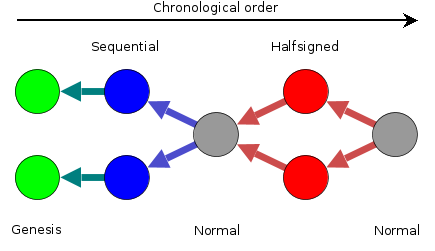
\includegraphics[scale=0.6]{experimentation/example.png}}
	\caption{Example of coloring used in Figures with graphs.}
	\label{fig:graph-example}
\end{figure}

Some experiments were also run multiple times because Dispersy does not always connect to every peer.
At the start of the experiment the peers are forced to be introduced,
but this does not always succeed.
This is a problem in discoverability and has been experienced by previous work aswell~\cite{ruigrok-anonymous}.
The final version is chosen when Dispersy did connect all the peers.
We recommend that Dispersy is changed to allow a modified behaviour when experimenting
where the pool of candidates is not refreshed,
as explained in section \ref{sect:bartercast}

\section{Software engineering tests}
MultiChain is tested in several ways to verify it is correctly working
following standard software engineering practices.
The enforcement of these types of tests is a policy recently introduced within Tribler.

\subsection{Unit Tests \& Integration tests}
Tribler uses Python unit tests to validate small components of code.
The tests can be run locally and
are automatically run on a Jenkins build server\cite{jenkins}\cite{jenkins-tribler}.
Unit tests were added to increase stability of MultiChain.
Integration tests were added to test multiple components of MultiChains working integrated together.

Tribler does prove to be hard to test using unit tests.
This is due to high coupling of code within Tribler.
But mocking of classes helped in testing difficult to test code.
The separate unit tests for the conversion, payload and database were the first of it types inside Tribler.
Also Dispersy was expanded to introduce new functionality to make it easier to create unit tests for communities in the future.
An overview of the coverage can be seen in Table \ref{tab:tests}
In the end a high level of testing has been achieved, especially in comparison to the rest of Tribler.
The total test coverage of Tribler was only 16\% at time of writing\cite{jenkins-tribler}.
A decision using code coverage tools was made that the untested code has little value to further test in comparison to the work required.
The code was tested in Gumby scenarios.

\begin{table}
\centering
\begin{tabular}{l|ll|ll}
Filename   & LOC & \% covered   & Conditionals & \% covered    \\ \hline
Community  & 187 & 81\%         & 37           & 95\%  \\
Conversion & 60  & 100\%        & 6            & 100\%  \\
Database   & 100 & 100\%        & 6            & 84\%  \\
Payload    & 89  & 100\%        & 2            & 100\% \\ \hline
Total      & 672 &              & 47           &
\end{tabular}
\caption{Unit tests coverage of MultiChain.}
\label{tab:tests}
\end{table}

\subsection{Gumby}

Next to that, Tribler uses a homemade test runner Gumby.
Gumby can start multiple instances of Tribler and follow test scenarios.
Gumby can be used to perform system tests and experiments.
These system tests have to be manually validated.
Several scenarios have been written to validate MultiChain.
These run MultiChain either in a standalone version or integrated into the TunnelCommunity.

One of these scenarios can be found in Figure \ref{fig:exp-gumby-scenario}
In this example basic block creation is tested.
Normal situations are tested,
but also situations where the signature requests are answered late
and other requests arrive at the requesting peer at the same time.
Additionally, signature requests are controlled to not be answered at all.
During the whole test the crawler is active and scrapes the network for unknown blocks.
The notation in the scenario is the time an action has to be taken place,
the action that has to be taken, and by who if necessary.
The "@0:" can be ignored, but is required in the Gumby format.

\begin{figure}
\begin{FVerbatim}[fontsize=\small]
@0:0 set_master_member 3081a7301006072a8648ce ... 2b51
@0:0 set_community_class MultiChainNoResponseCommunity {4}
@0:0 set_community_class MultiChainDelayCommunity {5}
@0:0 set_community_class MultiChainCommunityCrawler {6}
@0:0 set_community_class {6}
@0:0 start_dispersy
@0:1 online
@0:5 reset_dispersy_statistics
@0:10 annotate start-experiment-1-peer
@0:15 introduce_candidates
@0:80 request_signature 2 {1}
@0:84 request_signature 1 {2}
@0:94 request_signature 4 {1}
@0:95 request_signature 1 {3}
@0:104 request_signature 5 {1}
@0:106 request_block 1 5 {6}
@0:110 close
@0:111 stop_dispersy
@0:112 stop
\end{FVerbatim}
    \caption{One of the Gumby definition files.}
    \label{fig:exp-gumby-scenario}
\end{figure}

\section{Tracking download and upload amounts}
In this section we will experiment with MultiChain creating blocks and tracking download and upload amounts of peers.
We will first start with creating a simple block in an experiment.
The next experiment is to try to create a chain of blocks with mimicking a download of 10MB
and a larger download of 10GB.
Downloads are done at different download speeds and an experiment was done to test MultiChain in this environment.

\section{Single block creation}
In this experiment we try to create a block between two nodes.
This experiment validates the MultiChain to be able to correctly create a block between nodes in normal circumstances.
The experiment is locally run using gumby with all nodes running on a single computer.
Only two instances of MultiChain communities are started and between these two communities a block is created.
The logging of the both nodes is captured and recorded to verify the results of the experiment.

The output of the logging can be seen in figure \ref{fig:singleblockexperiment}.
First node 1 sends a signature request to node 2.
This message is received and a block is persisted.
The hash of the block is displayed in the output.
The block is sent back as a signature response to node 1.
The block is saved by node 1 and has the same hash as shown in the output.
So the block between node 1 and node 2 is the same and a block was succesfully created.
The output also shows behaviour of MultiChain
to correctly exclude any other execution from entering mutual exclusive code.
The lines related to the mutual exclusion are prepended by "Chain Excl".
The nodes check if it is possible to enter the mutual exclusive part and correctly acquires
and releases the mutual exclusion token.

\begin{figure}
\begin{FVerbatim}[fontsize=\small]
1: Requesting Signature for candidate: 2
1: Chain Exclusion: signature request: False
1: Chain Exclusion: acquired, sending signature request.
1: Sending signature request.
2: Received signature request.
2: Chain Exclusion: process request: False
2: Chain Exclusion: acquired to process request.
2: Persisting sr: 2F7bTMxyJU7hZkvaBimT2bYm4bY=
2: Chain Exclusion: released after processing request.
2: Sending signature response.
1: Signature response received. Modified: True
1: Valid 1 signature response(s) received.
1: Persisting sr: 2F7bTMxyJU7hZkvaBimT2bYm4bY=
1: Chain exclusion: released received signature response.
\end{FVerbatim}
    \caption{Output of single block creation experiment}~\label{fig:singleblockexperiment}
\end{figure}

\subsection{Chaining blocks}
The next experiment we experiment with MultiChain creating a chain of blocks between two peers.
The experiment is run using gumby with all peers running on a single computer.
We try to create 10 subsequent blocks mimicking a download of 10MB with a speed of 1000 KB/s.
Every second these amounts are indicated to have been transferred to the schedulers of every peer.
The scheduler waits for 1MB uploaded to another peer before scheduling a block.

The result of the experiment can be seen in the graph in Figure \ref{fig:chain-experiment-graph}.
In this graph it can be clearly seen that MultiChain is succesful in creating a chain of 10 blocks.

\begin{figure}[!h]
	\centerline{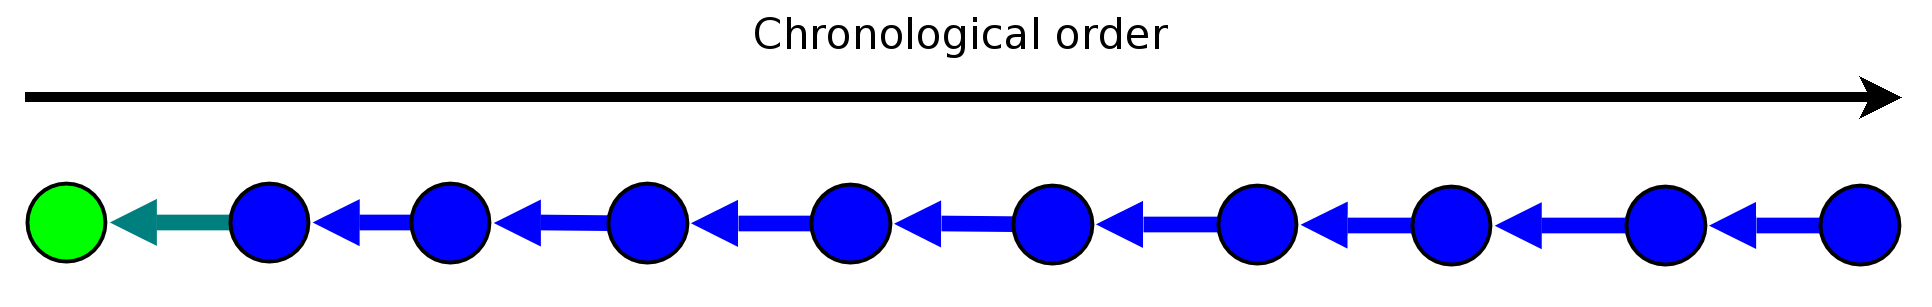
\includegraphics[scale=0.6]{experimentation/chain/chain.png}}
	\caption{MultiChain chain graph of a single download of 10 MB.}
	\label{fig:chain-experiment-graph}
\end{figure}

The amounts stored in each blocks are plotted in Figure \ref{fig:chain-experiment-amounts}.
Every datapoint is a block in the chain of a peer and is the the total amount stored in that block..
These datapoints are connected by a dotted line representing the link between these blocks.
These plots show that MultiChain correctly tracks the download of 10MB.
The slope of the figure corresponds with the speed of the download.

\begin{figure}
\centering
\subfigure[Total download amount.]{
\centerline{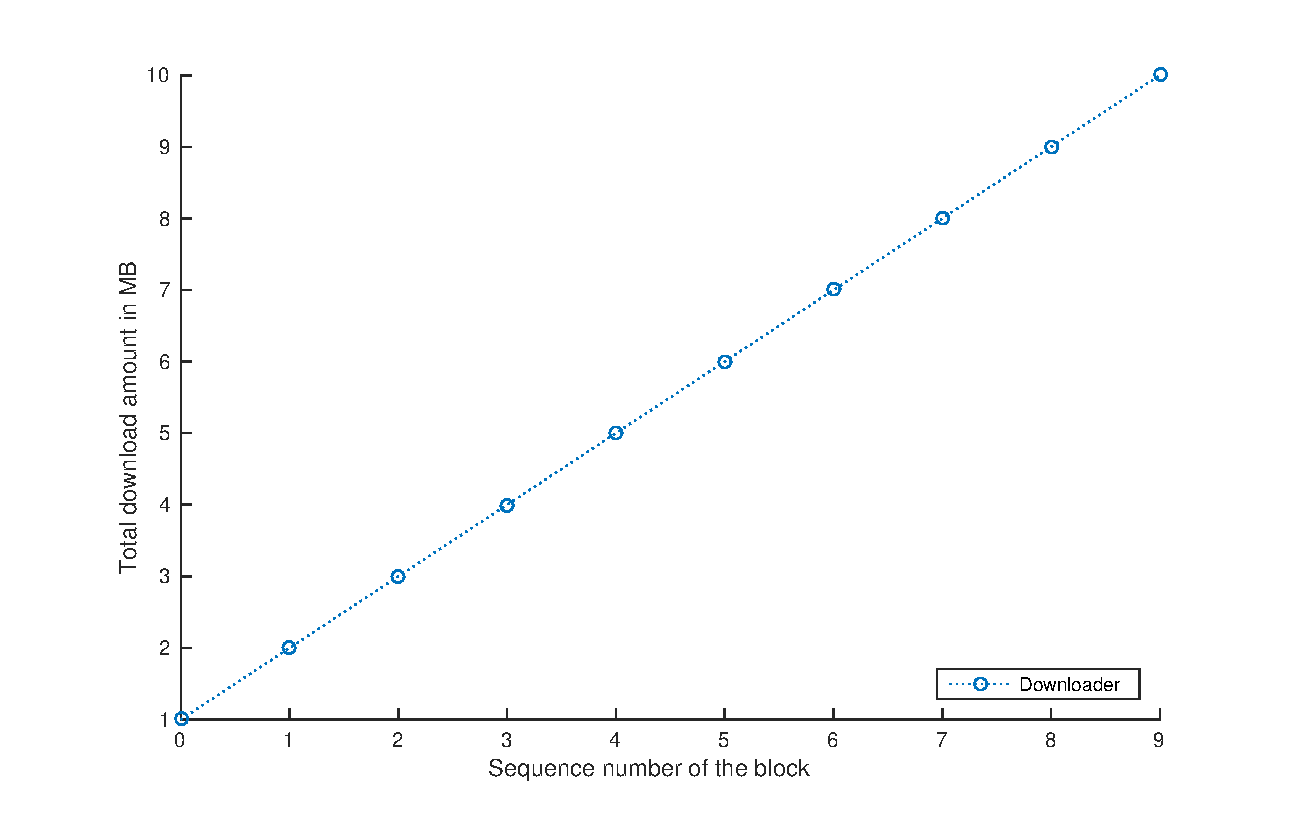
\includegraphics[scale=0.5]{experimentation/chain/chain-down.eps}}
\label{fig:chain-experiment-down}
}
\subfigure[Total upload amount.]{
\centerline{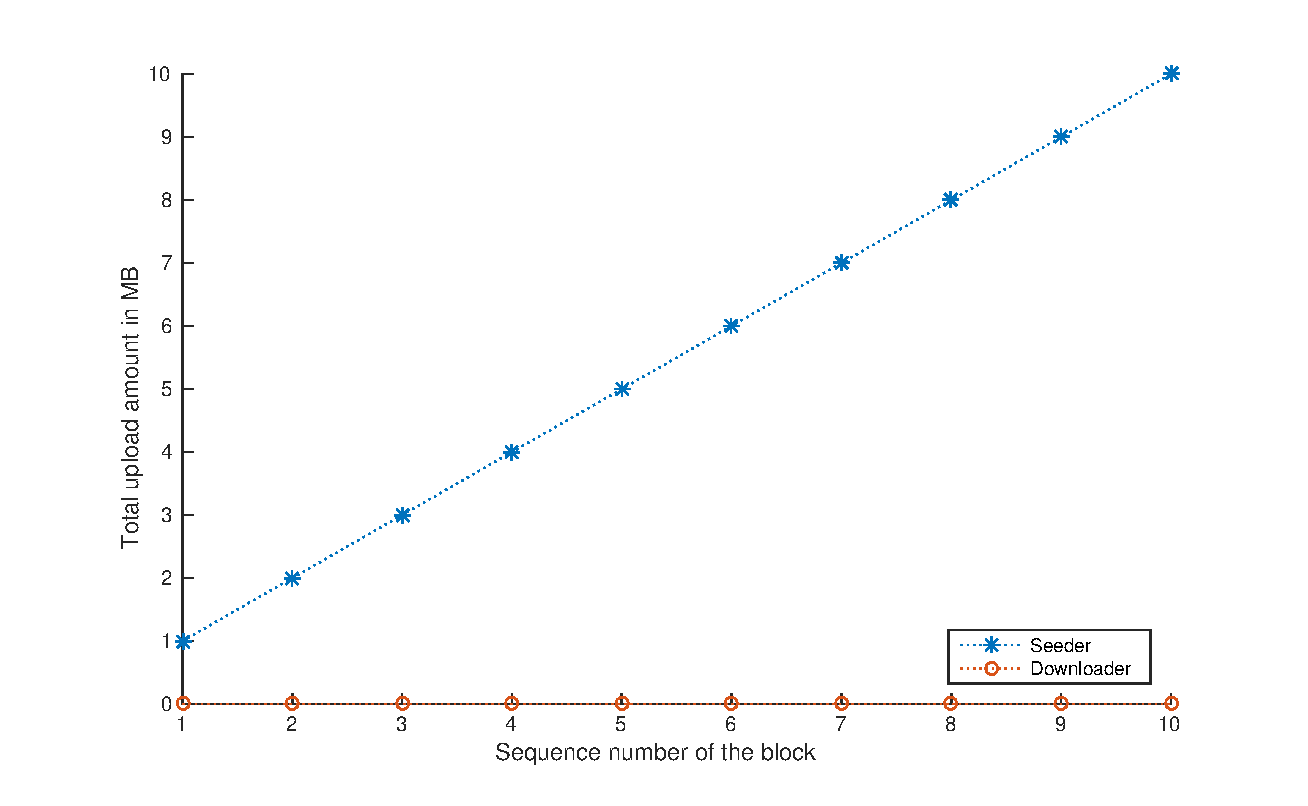
\includegraphics[scale=0.5]{experimentation/chain/chain-up.eps}}
\label{fig:chain-experiment-up}
}
\caption{Download and upload amounts when creating a chain of 10 blocks.}
\label{fig:chain-experiment-amounts}
\end{figure}

\subsection{Tracking downloads with different speeds}
In this experiment we measure if MultiChain can correctly track the upload and download amounts
between two peers with different speeds.
In the scenario a file of 100 MB is downloaded at different speeds,
respectively 500 KB/s, 750 KB/s, 1000 KB/s, 1250 KB/s, 2000 KB/s, and 3000 KB/s.
The maximum speed of anonymous download was measured in experiments to be 1150 KB/s\cite{ruigrok-anonymous}.
The scheduler waits for 1MB uploaded to another peer before scheduling a block.
The upload and download of the file is done by different pairs of seeders and leechers.
Every second these amounts are indicated to have been transferred to the schedulers of every peer.

\begin{figure}
\centering
\subfigure[Total download amount.]{
\centerline{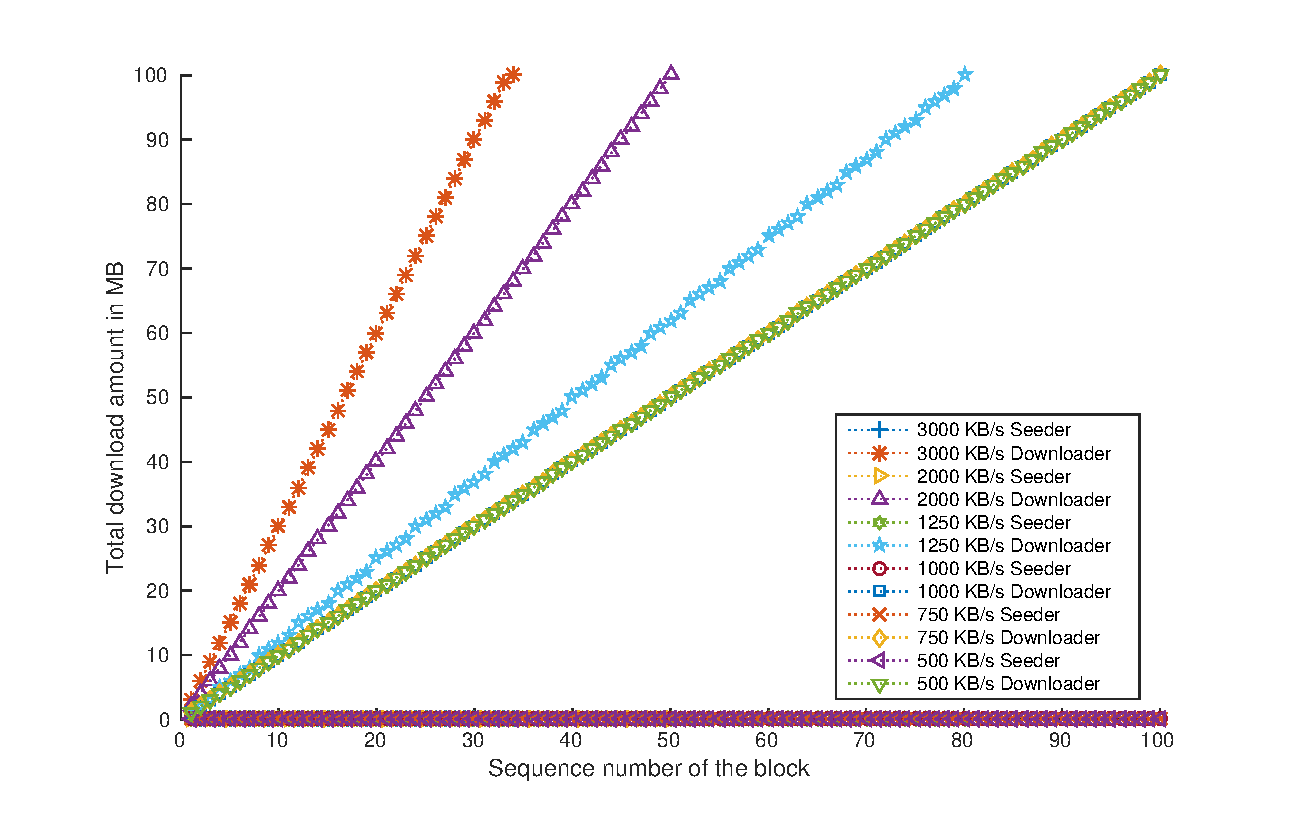
\includegraphics[scale=0.5]{experimentation/speeds/synthetic-simple-down.eps}}
\label{fig:synthetic-simple-down}
}
\subfigure[Total upload amount.]{
\centerline{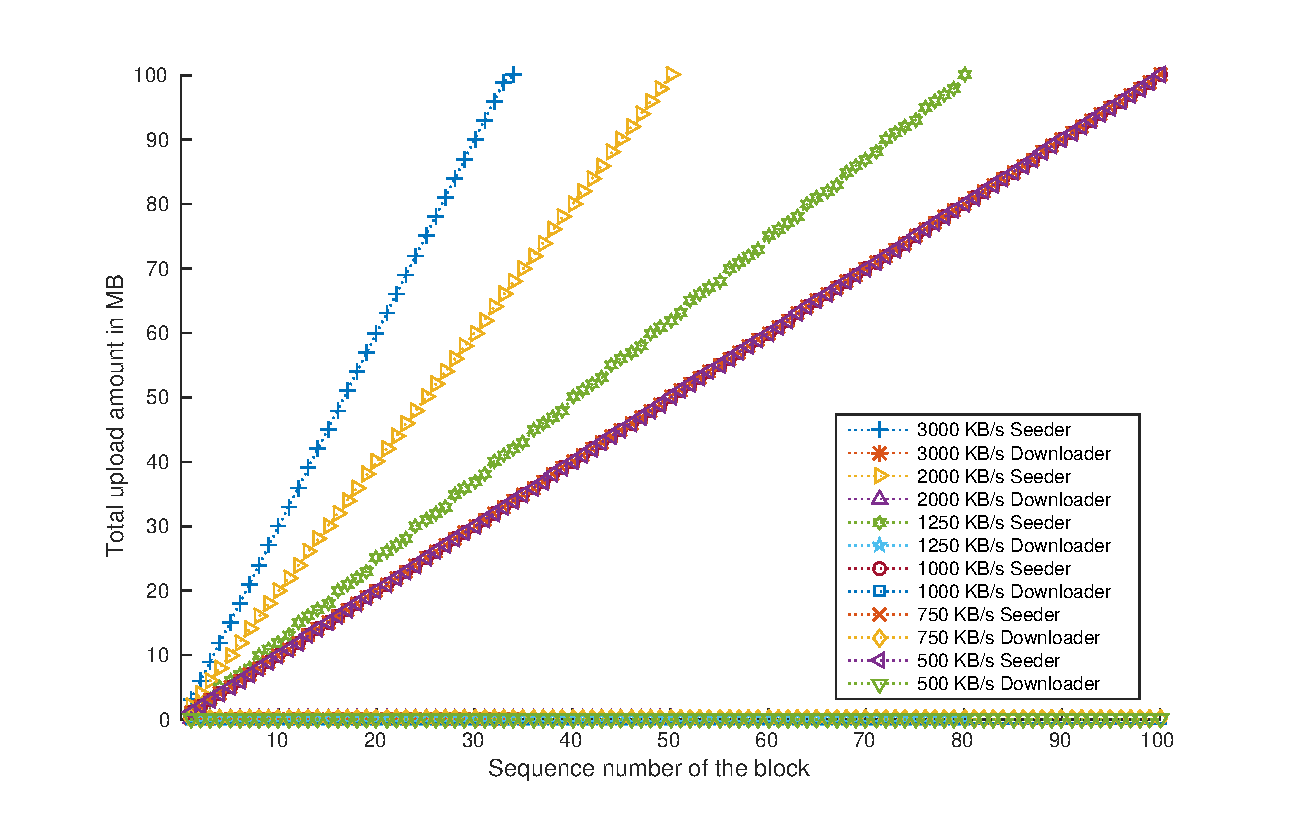
\includegraphics[scale=0.5]{experimentation/speeds/synthetic-simple-up.eps}}
\label{fig:synthetic-simple-up}
}
\caption{Download and upload amounts when tracking downloads at different speeds.}
\label{fig:synthetic-simple-amounts}
\end{figure}

The total download and upload amounts of every peer is plotted in Figure \ref{fig:synthetic-simple-amounts}.
These amounts are plotted in the same way as the previous experiment.
The plots show that MultiChain is able to correctly track the download and upload amounts without a problem.
There are no hitches in the figures and the amounts go up in fixed increments corresponding to the different speeds.
This means that MultiChain is fast enough to correctly track the amounts.

The download speeds below the threshold of 1000 MB of the scheduler
are not distinguishable from the download at the threshold speed.
This is because the scheduler waits until the threshold is reached before initiating the block.
The amount is tracked in the same amount of blocks,
but the total time of the experiment is longer for these experiments.
If the speed goes above the threshold, then this is reflected in the figure.

The graph in Figure \ref{fig:synthetic-simple-graph} shows the graph of the blocks created by the experiment.
The graph is disconnected, because the different pairs of seeders and leechers did not interact with each other.
So no block that would connect their chains is created,
This leaves the graph disconnected.

\begin{figure}
	\centerline{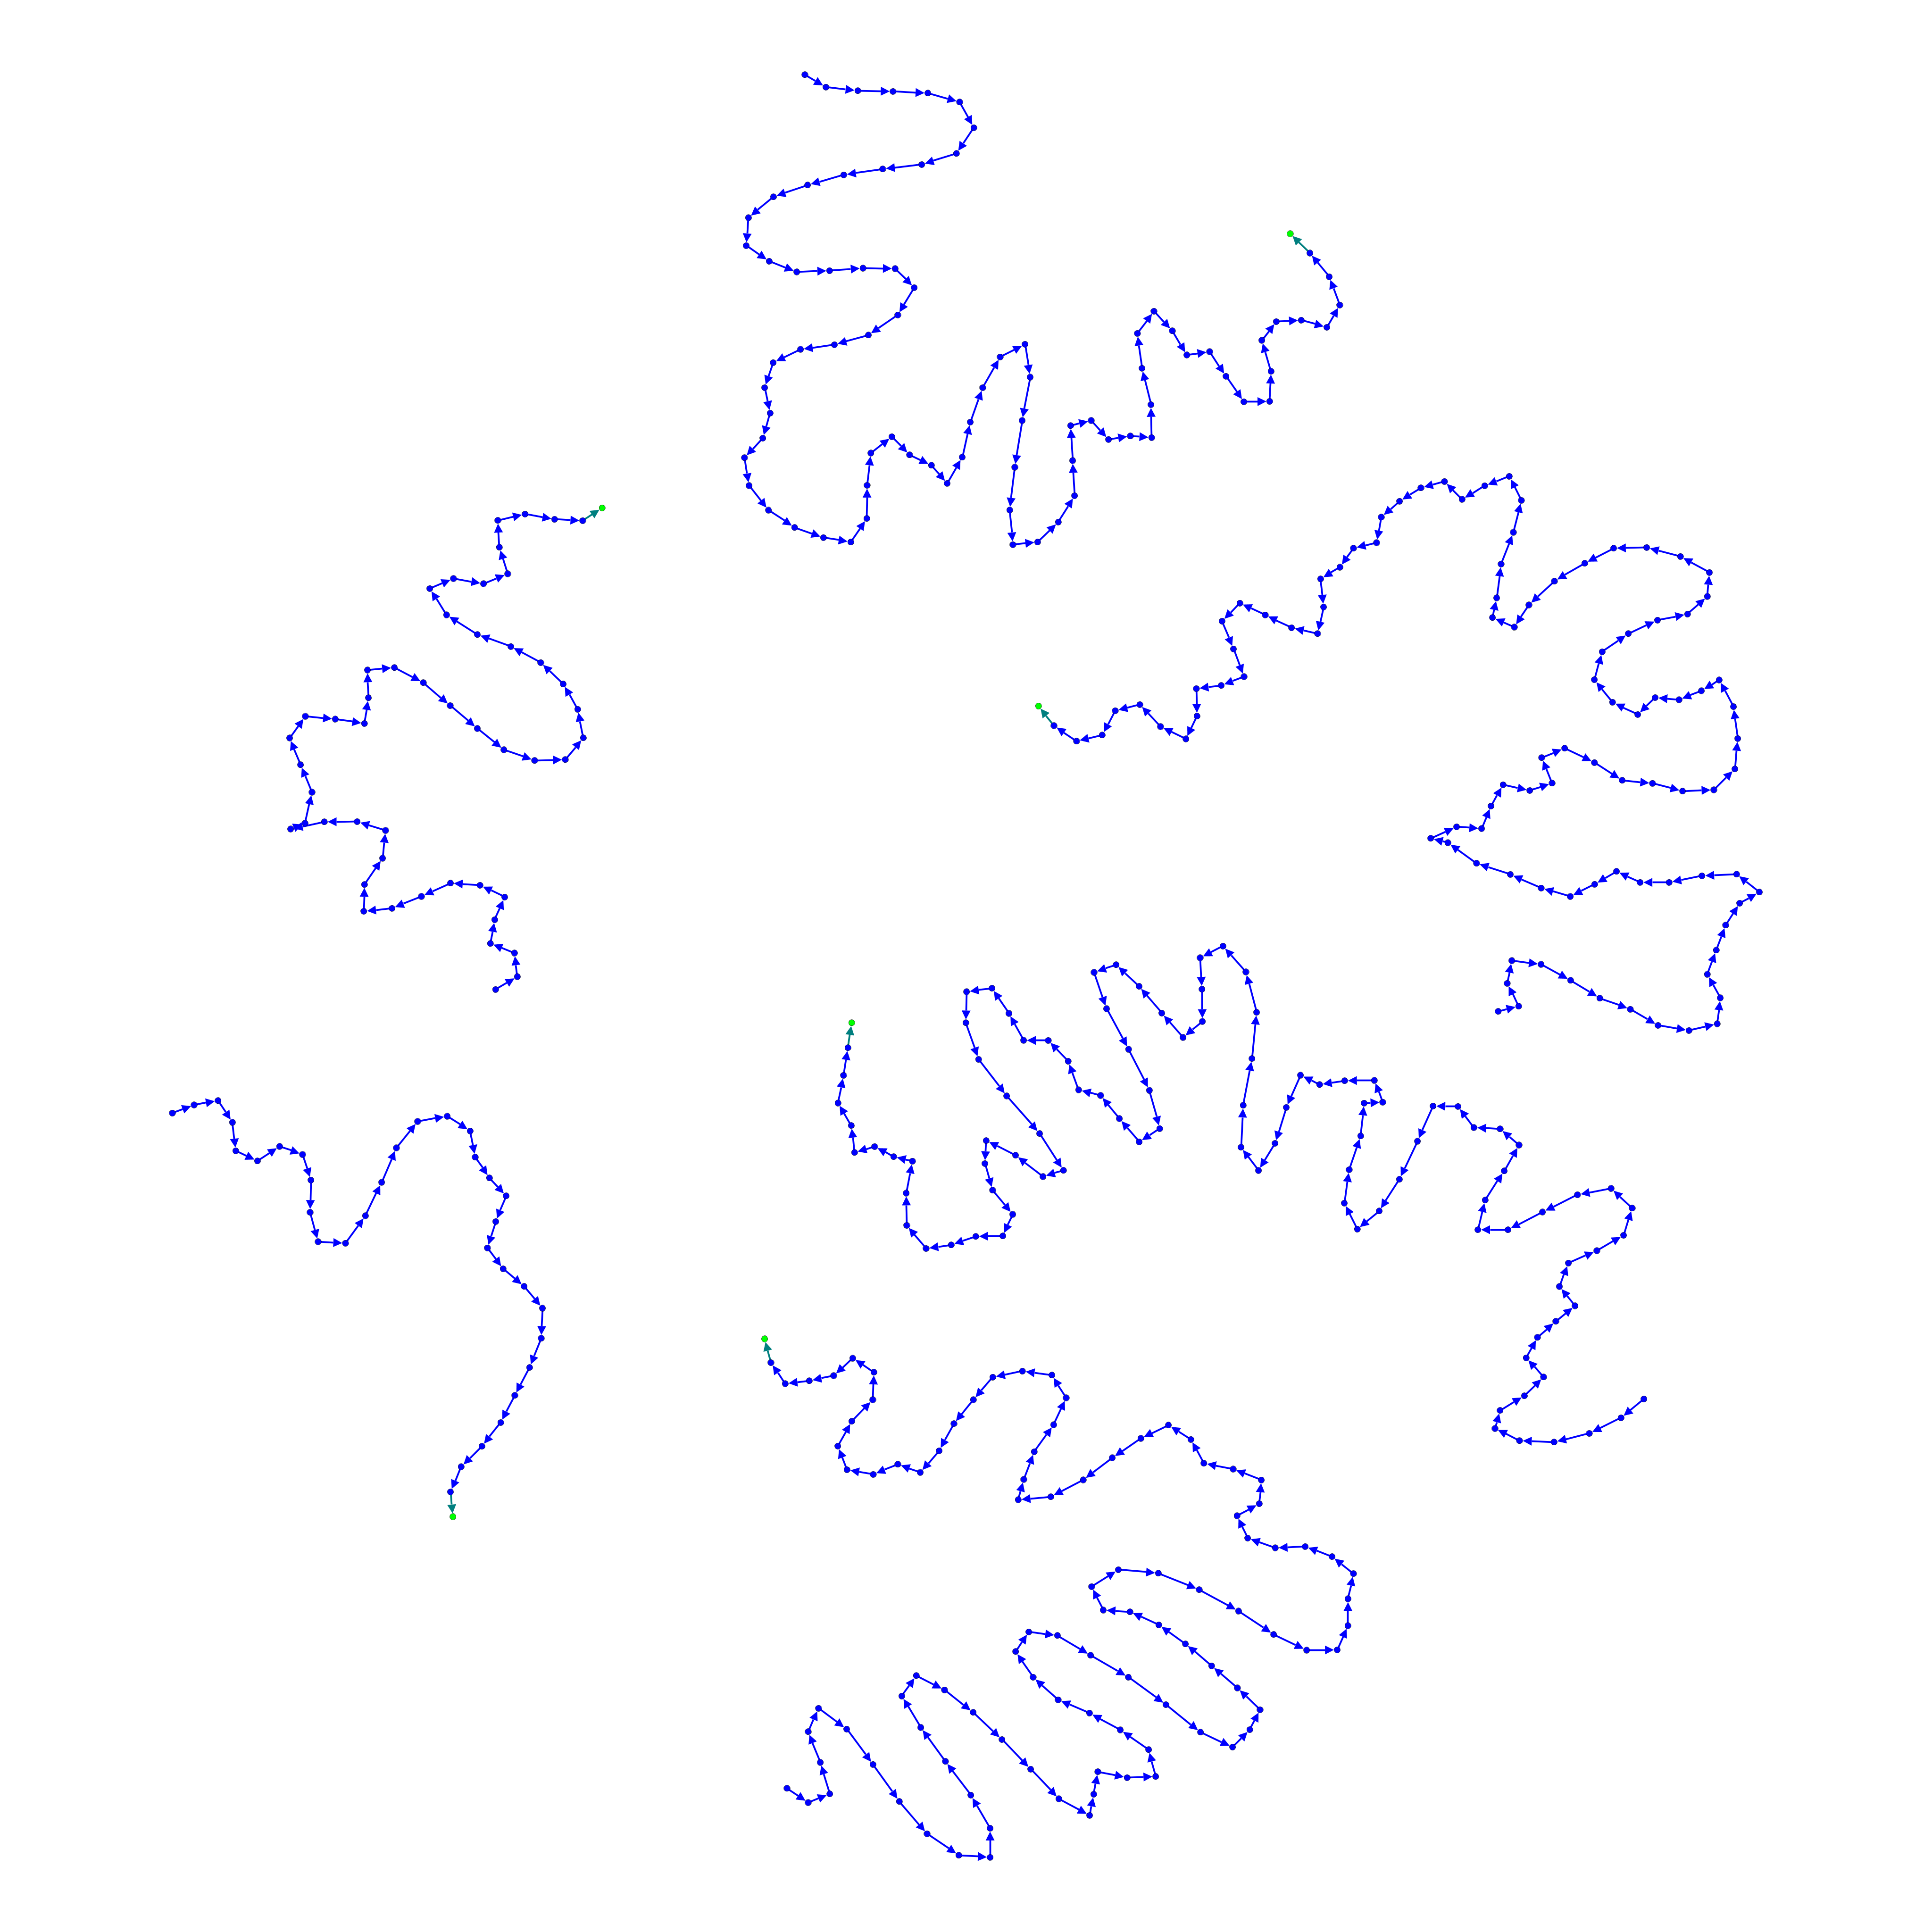
\includegraphics[scale=0.06]{experimentation/speeds/synthetic.png}}
	\caption{Disconnected chain graph of 6 individual downloads at different speeds.}
	\label{fig:synthetic-simple-graph}
\end{figure}

This experiment was run several times before the final version in this report was run.
Earlier versions of the experiment resulted in two bugfix and two improvements:
the ability of the scheduler to create a block at the end of a download.

\section{Tracking anonymous data transfer}
In this section we will experiment with MultiChain tracking anonymous data transfer.
Anonymous data transfer is a more complicated environment,
where multiple peers work together to transfer data from the seeder to the leecher.
We experiment in a synthetic environment and in environment using real anonymous downloads between peers.

\subsection{Anonymous download}
In an anonymous download scenario the data is downloaded through multiple hops.
A seeder uploads data to the first hop.
This hop passes the data to the second hop.
The second hop sends the data to its destination at the leecher.
This can be seen as sequence of peers and is illustrated in Figure \ref{fig:seeder-hops-leecher}.
More hops can be added to better safegaurd the anonymity of the download.

\begin{figure}
	\centerline{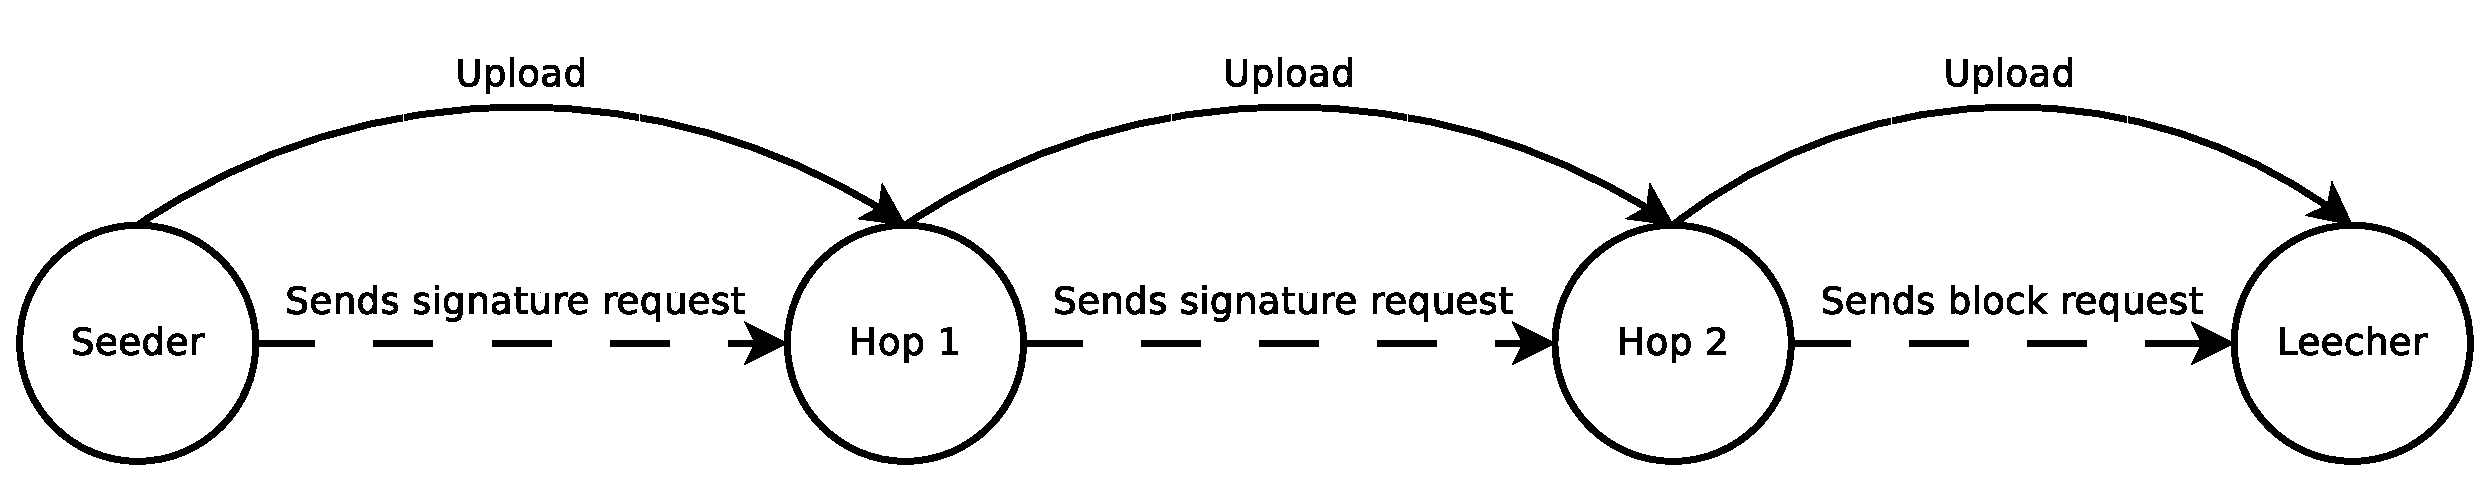
\includegraphics[scale=0.3]{experimentation/anonymous/seeder-hops-leecher.eps}}
	\caption{Block creation in an anonymous download.}
	\label{fig:seeder-hops-leecher}
\end{figure}

The total download and upload amount is plotted, in the same way as the previous experiment,
in Figure \ref{fig:synthetic-anonymous-amounts}.
The slopes of the figures are not representative for the upload and download speeds of the peers.
This is because the x-axis represents the sequence-number of the block and not time.
The hops create blocks that can be categorized in two types:
a download validating block and an upload validating block.
The download validating block only contains information about how much the hop has downloaded
and is initiated by the peer in front of the peer in the sequence.
An upload validating block is initiated by the peer itself with the peer next in the sequence.
The seeder only has upload validating blocks and as such has half the amount of blocks.
The downloader has viceversa only download validating blocks.
The slope of his figure is much steeper as a result.

In the graph a hitch can be found in the figures of the seeder and the first hop.
This is the result of the first hop sending a signature request to the second hop.
The second hop was not able to process this request,
because it was already working on creating another block.
The first hop will still wait on the second hop to process its request untill it will timeout.
In turn, the seeder sent a request to the first hop that will timeout,
because the first hop is not able to process this request aswell.
During the timeouts of the seeder and the first hop,
the second hop continues to validates its own upload amounts.
No blocks are created that validate his download amount,
so the slope becomes steeper during that time and the download amount remains level.
The timeouted peers create no blocks.
When the timeouts expires, the system returns to function as normal.
In section \ref{sect:deadlock-exp} we further experiment with the timeouts in the system.

\begin{figure}
\centering
\subfigure[Total download amount.]{
\centerline{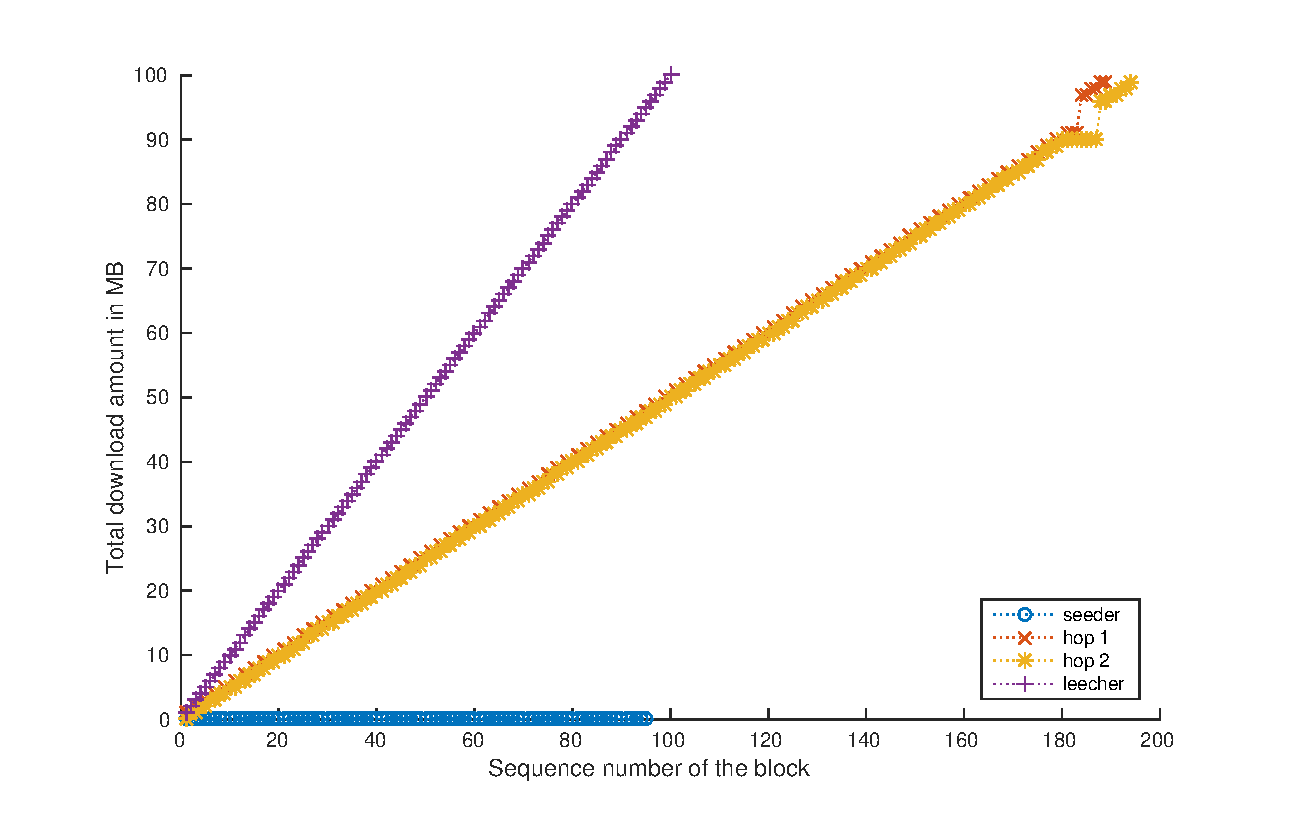
\includegraphics[scale=0.5]{experimentation/anonymous/synthetic-anonymous-down.eps}}
\label{fig:synthetic-anonymous-down}
}
\subfigure[Total upload amount.]{
\centerline{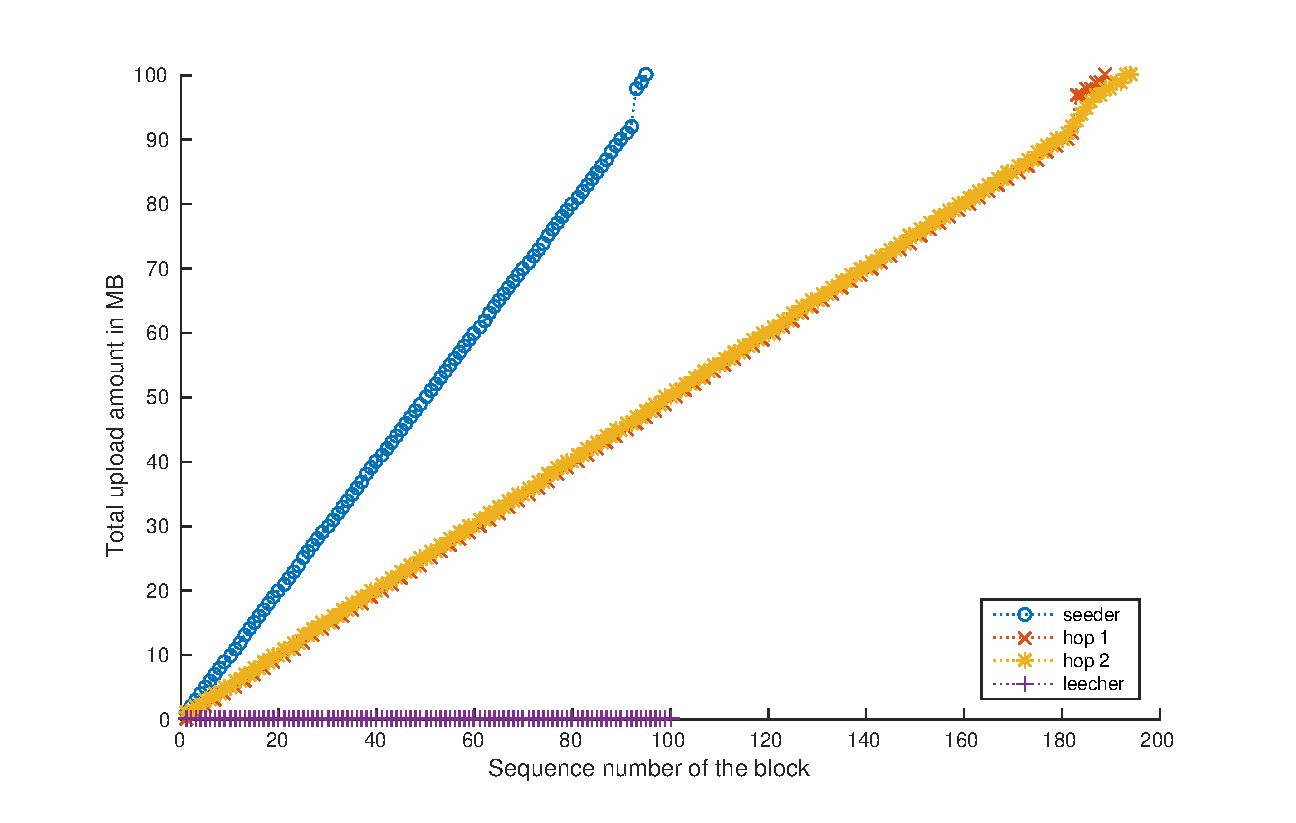
\includegraphics[scale=0.5]{experimentation/anonymous/synthetic-anonymous-up.eps}}
\label{fig:synthetic-anonymous-up}
}
\caption{Download and upload amounts during the anonymous download experiment.}
\label{fig:synthetic-anonymous-amounts}
\end{figure}

The graph in Figure \ref{fig:synthetic-anonymous-graph} shows the graph of the blocks created by the experiment.
In contrast to the previous experiment, this graph is connected.
Because every peer interacts indirectly with every other peer.

\begin{figure}
	\centerline{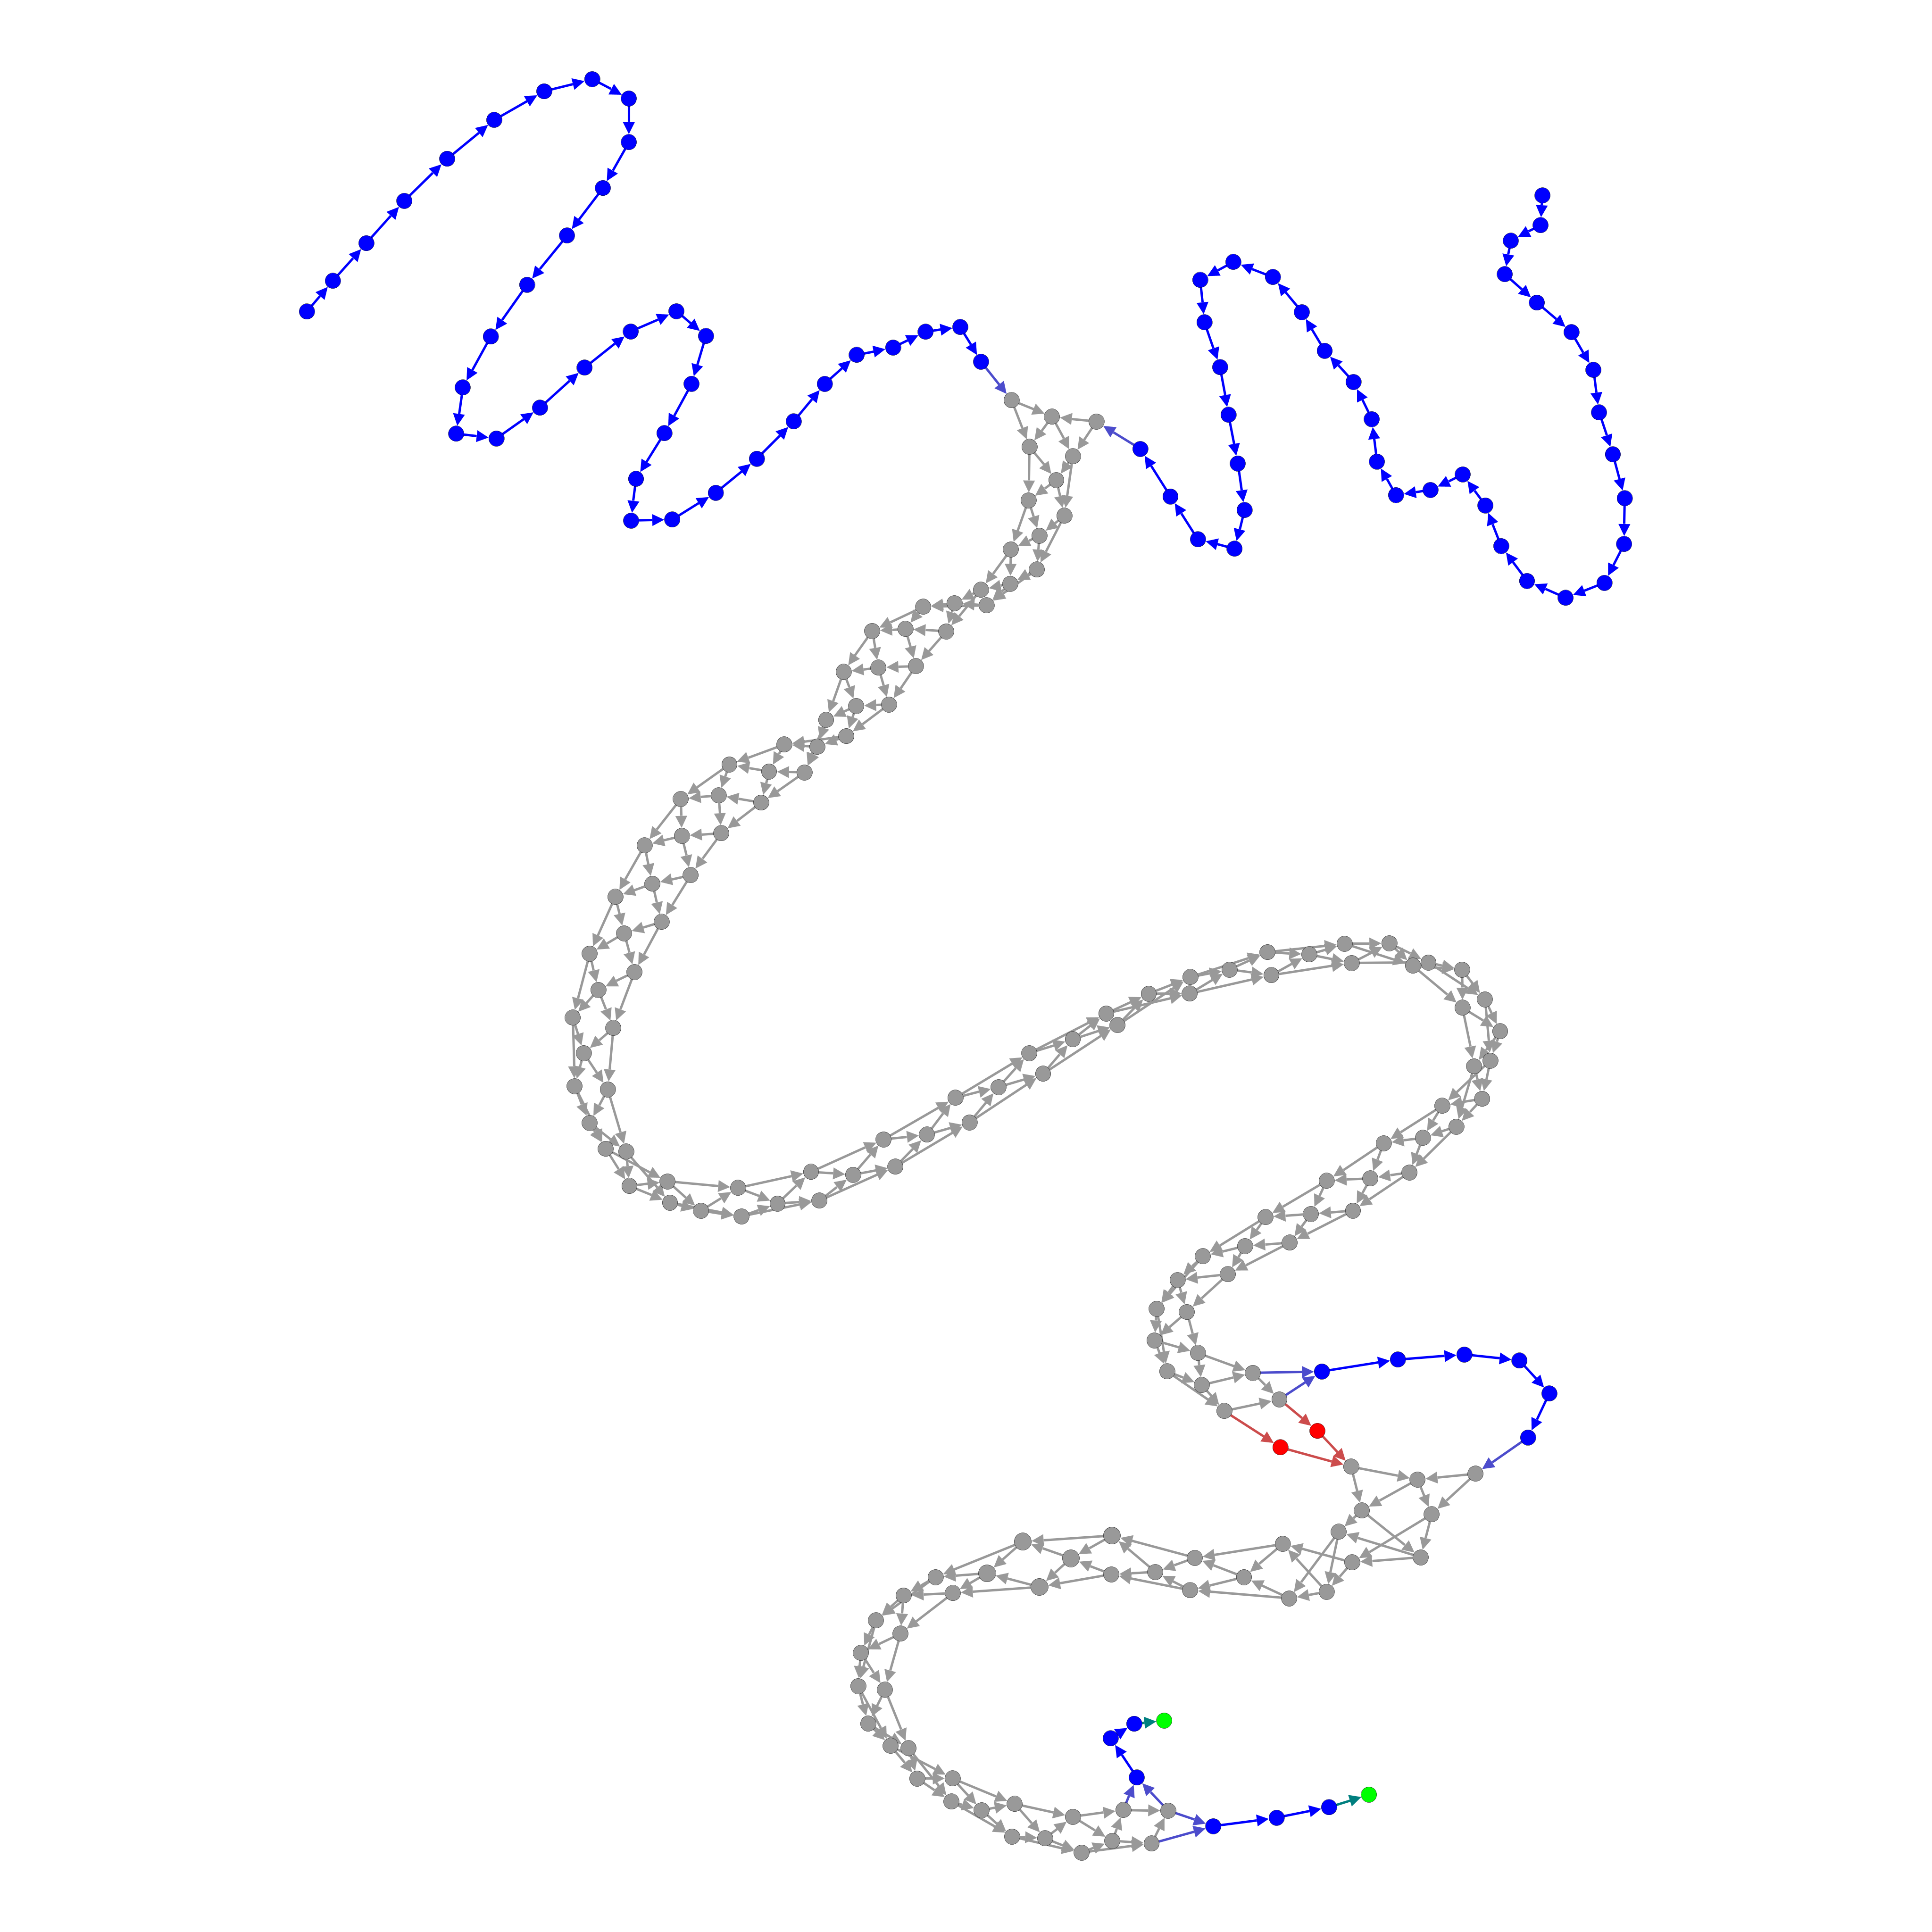
\includegraphics[scale=0.1]{experimentation/anonymous/anonymous.png}}
	\caption{MultiChain chain graph of a single download through 2 hops.}
	\label{fig:synthetic-anonymous-graph}
\end{figure}

The seeder and leecher both only interact with one hop.
These hops furthermore only interact with each other.
This can be clearly seen a part of the graph magnified in Figure \ref{fig:synthetic-anonymous-graph-magnified}.
The middle nodes represent the interaction between the hops.
The outer nodes are interactions between the seeder and the first hop and between the second hop and leecher.
The blocks are created alternating resulting in the graph pictured.

\begin{figure}
	\centerline{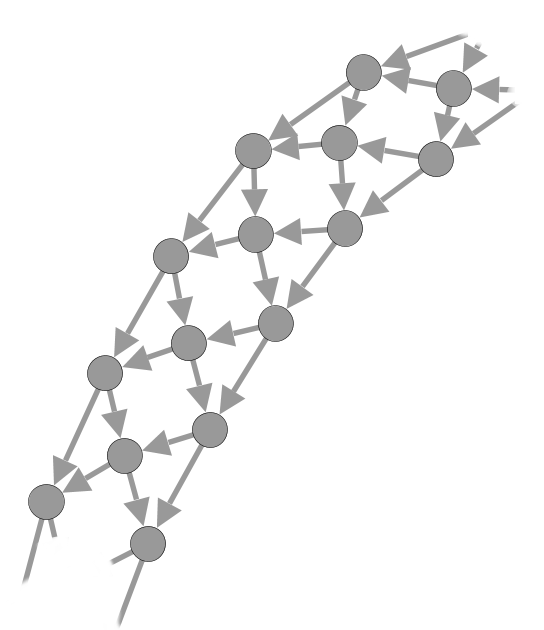
\includegraphics[scale=0.5]{experimentation/anonymous/anonymous-magnified.png}}
	\caption{Magnification of part of the graph.}
	\label{fig:synthetic-anonymous-graph-magnified}
\end{figure}

In the graph the timeout period can be seen clearly in Figure \ref{fig:synthetic-anonymous-graph}.
The two half-signed block can be seen in red.
The block with a reference coming from the outer block is the half-signed block belonging to the seeder.
The strain of blue nodes are the blocks created between the second hop and the leecher.
The red inner block is referenced by the first block created between the first hop and second hop after the timeout.






\subsection{Integrated anonymous download}
An substantial effort was made to integrated the tunnel community and hidden services community with the MultiChain community.
These communities work together to provide functionality to transfer data anonymously.
The tunnel community reports data transferred between peers and the MultiChain community add these amounts to the chain.
They are already integrated with BarterCast.
The method of integration of BarterCast was used to try to integrated MultiChain aswell.
Setting up the Gumby environment to run all communities took also considerable time.

Experiments were conducted where an 100 MB file is transferred by the actual anonymity communities,
while MultiChain transcribes the transfer amounts in the MultiChain.
The first experiment we ran was to test the integration without any hops.
In this setup the integration does not report any data transferred between the peers.
As such the scheduler never sees a reason to schedule a signature request.
The whole MultiChain community is never active.
MultiChain should also track these downloads,
but this requires MultiChain to be integrated in different places.

The second experiment was conducted with 2 hops.
The result of the experiment can be seen in Figure \ref{fig:integrated-anonymous-amounts}.
This shows that MultiChain does track the amount of upload and download for all peers in the network.
The hops roughly download and upload the same amount of their data.
This is what we expected as they just relay the data.
The seeder and downloader respectively only uploads and downloads.

Timeouts can be seen in the plots where the plot discontinues and does not grow steadily.
The reason these timeouts occur is that thresholds of the scheduler of every node is now reached at the same time resulting in a timeout.
Our recommendation is to have these thresholds to be shifted by a small amount randomly for every peer
to prevent them from overlapping.

\begin{figure}
\centering
\subfigure[Total download amount.]{
\centerline{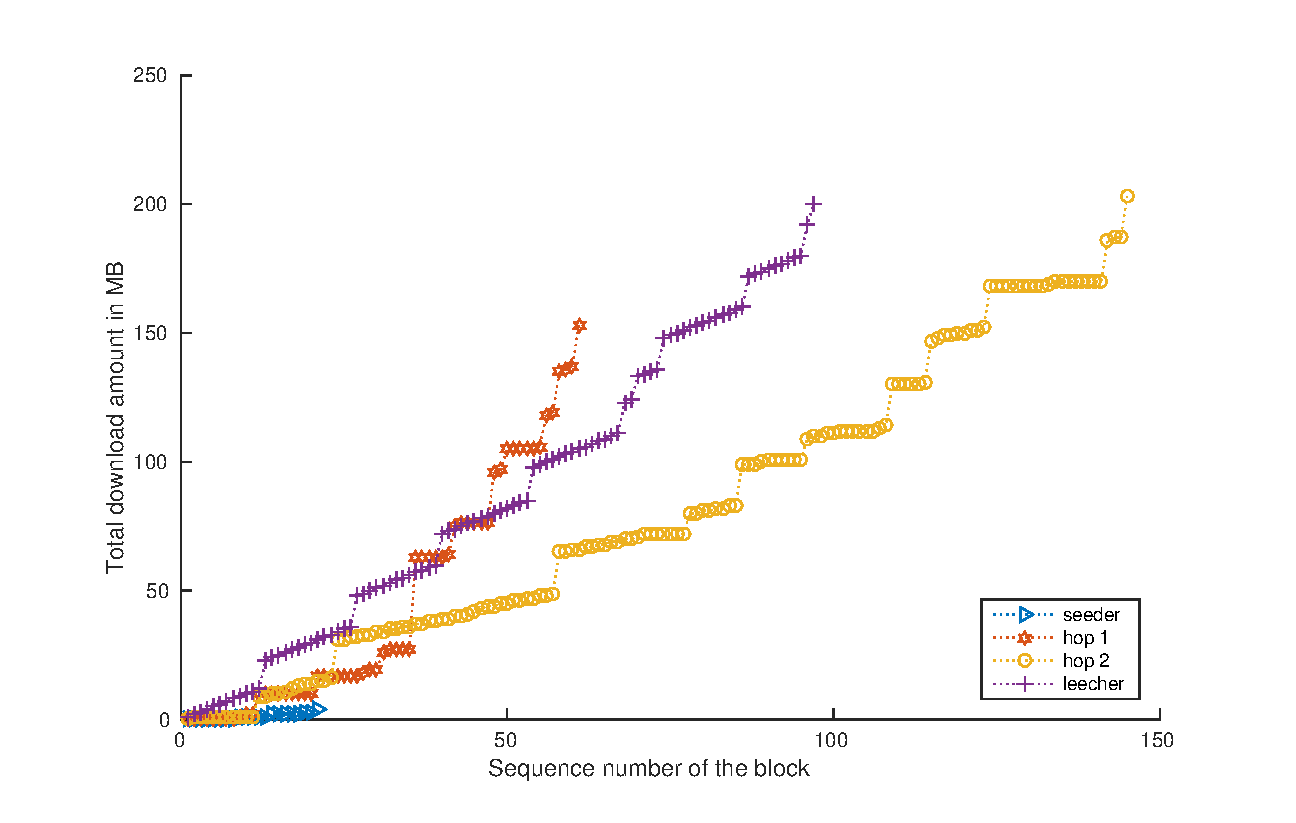
\includegraphics[scale=0.5]{experimentation/anonymous-integrated/integrated-anonymous-down.eps}}
\label{fig:integrated-anonymous-down}
}
\subfigure[Total upload amount.]{
\centerline{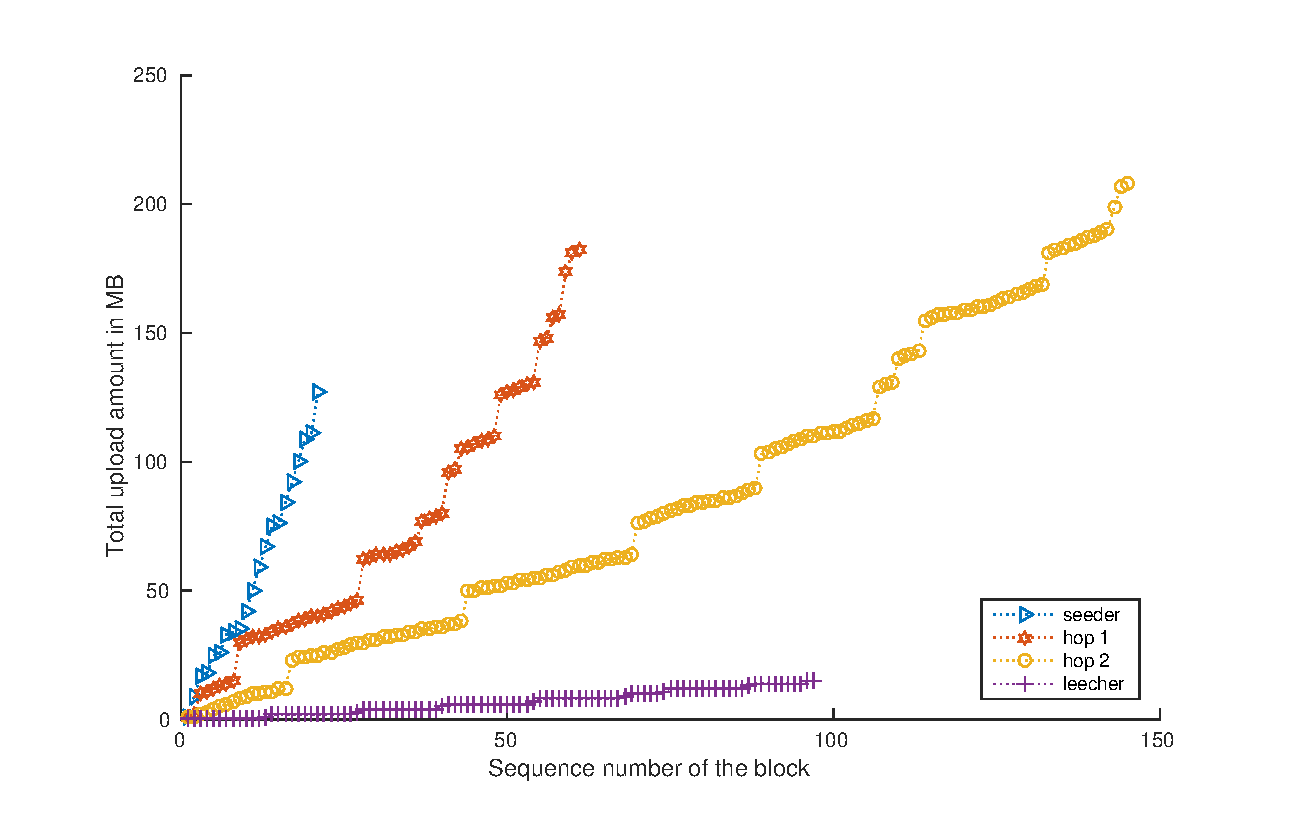
\includegraphics[scale=0.5]{experimentation/anonymous-integrated/integrated-anonymous-up.eps}}
\label{fig:integrated-anonymous-up}
}
\caption{Download and upload amounts during the integrated anonymous download experiment.}
\label{fig:integrated-anonymous-amounts}
\end{figure}

The amount of data that is reported to be transferred is remarkable.
The overhead measures twice the actual download size.
We therefore the conclusion that the integration is not properly and too much data is reported.
It is unclear where this data originates from.

Integrating MultiChain into the anonymous download communities is difficult,
because those communities do not use the standard classes used by Tribler to send messages.
These are necessary to properly integrate MultiChain and a complicated conversion was necessary.
Our recommendation is to refactor the anonymous download communities to use the standard classes
and to make it more clear in the code where data is sent and where data is received.
Also comments should be added to clarify the code.
Currently, there are no comments whatsoever.
This effort should atleast clarify why so much data is reported and will probaly fix the problem.

\section{Drop event recovery}
\label{sect:deadlock-exp}
MultiChain can run during normal operation into a situation
where a multiple of peers request to create blocks from each other as explained in section \ref{sect:deadlock}.
A specific experiment was conducted that created the situation manually.
This situation was also encountered during experimentation
and the experiment shows MultiChain correctly recovering from this situation.

\subsection{Forced drop event}
In this experiment a MultiChain node 1 tries to send a request to node 2 to create a block.
Node 2 is specifically configured for the purpose of the experiment
to ignore and drop all requests.
Node 1 now should wait for the response of the other node for a specific time.
During the time that node 1 is waiting a different request is sent from a normal node 3 to node 1.
This request will be dropped by node 1,
as it cannot process any incoming requests while node 1 has an outstanding request.
Node 1 and node 2 should timeout and continue operations.
After that node 2 will retransmit a request to node 1 and this should be completed correctly.

The experiment is locally run using gumby with all nodes running on a single computer.
Only three instances of MultiChain communities are started.
One of these instances never respond to a request to construct a block.
The logging of the every node is captured and recorded to verify the results of the experiment.

The output of the logging can be seen in Figure \ref{fig:manual-deadlock-experiment}.
First node 1 sends a signature request to node 2.
This message is ignored by node 2.
During the waiting period of node 1 a block request is sent to node 1 by node 3.
This request is also ignored, because node 1 cannot perform operations on the chain.
After the timeout period both node 1 and node 2 save an half-signed block to their chain
and can continue operations.
This is validated by a block created between node 3 and node 1.

\begin{figure}
\begin{FVerbatim}[fontsize=\small]
1: Requesting Signature for candidate: 2
1: Chain Exclusion: signature request: False
1: Chain Exclusion: acquired, sending signature request.
1: Sending signature request.
2: Received signature request that will be ignored.

3: Requesting Signature for candidate: 1
3: Chain Exclusion: signature request: False
3: Chain Exclusion: acquired, sending signature request.
3: Sending signature request.
1: Received signature request.
1: Chain Exclusion: process request: True
1: Chain Exclusion: not acquired. Dropping request.

1: Timeout received for signature request.
1: Persisting sr: bFOXhHT2ffSrtIn9tuMfEGGarGY=
3: Timeout received for signature request.
3: Persisting sr: l1O8UquXdxWdkg+KAYZ1FYocwjo=
3: Requesting Signature for candidate: 1

3: Chain Exclusion: signature request: False
3: Chain Exclusion: acquired, sending signature request.
3: Sending signature request.
1: Received signature request.
1: Chain Exclusion: process request: False
1: Chain Exclusion: acquired to process request.
1: Persisting sr: 7Y86Ck4duwTduP6j/aIRrWHAZqw=
1: Sending signature response.
3: Signature response received. Modified: True
3: Valid 1 signature response(s) received.
3: Persisting sr: 7Y86Ck4duwTduP6j/aIRrWHAZqw=
3: Chain exclusion: released received signature response.
\end{FVerbatim}
    \caption{Output of the manual drop event experiment}~\label{fig:manual-deadlock-experiment}
\end{figure}

\subsection{Naturally occuring drop events}
In the experiment a 100 megabyte file was downloaded anonymously with 2 hops.
Anonymously downloading is described more in the thesis report of R. Ruigrok~\cite{ruigrok-anonymous}.
There are 2 Triblers instances with exit functionality and 18 instances without exit functionality.
All instances are run locally on one machine.
The instances are run in parallel,
so the fact that all instances are run on a single machine does not cause the drop event to occur.
There is no packetloss in this experiment.
The corresponding graph of all the MultiChains of the experiment can be seen in Figure \ref{fig:deadlock-double}.

The potential scenario of two peers both waiting can be seen multiple times in the graph and are encircled.
The scenario generates a half-signed block at both peers.
Usually the peers continue collaboration and this continuation of a sequence can be seen in subsequent blocks.
In the graph a more complicated scenario can also be seen where multiple peers timeout between each other.
The graph shows that MultiChain correctly recovers from all scenario's.

\begin{figure}
	\centerline{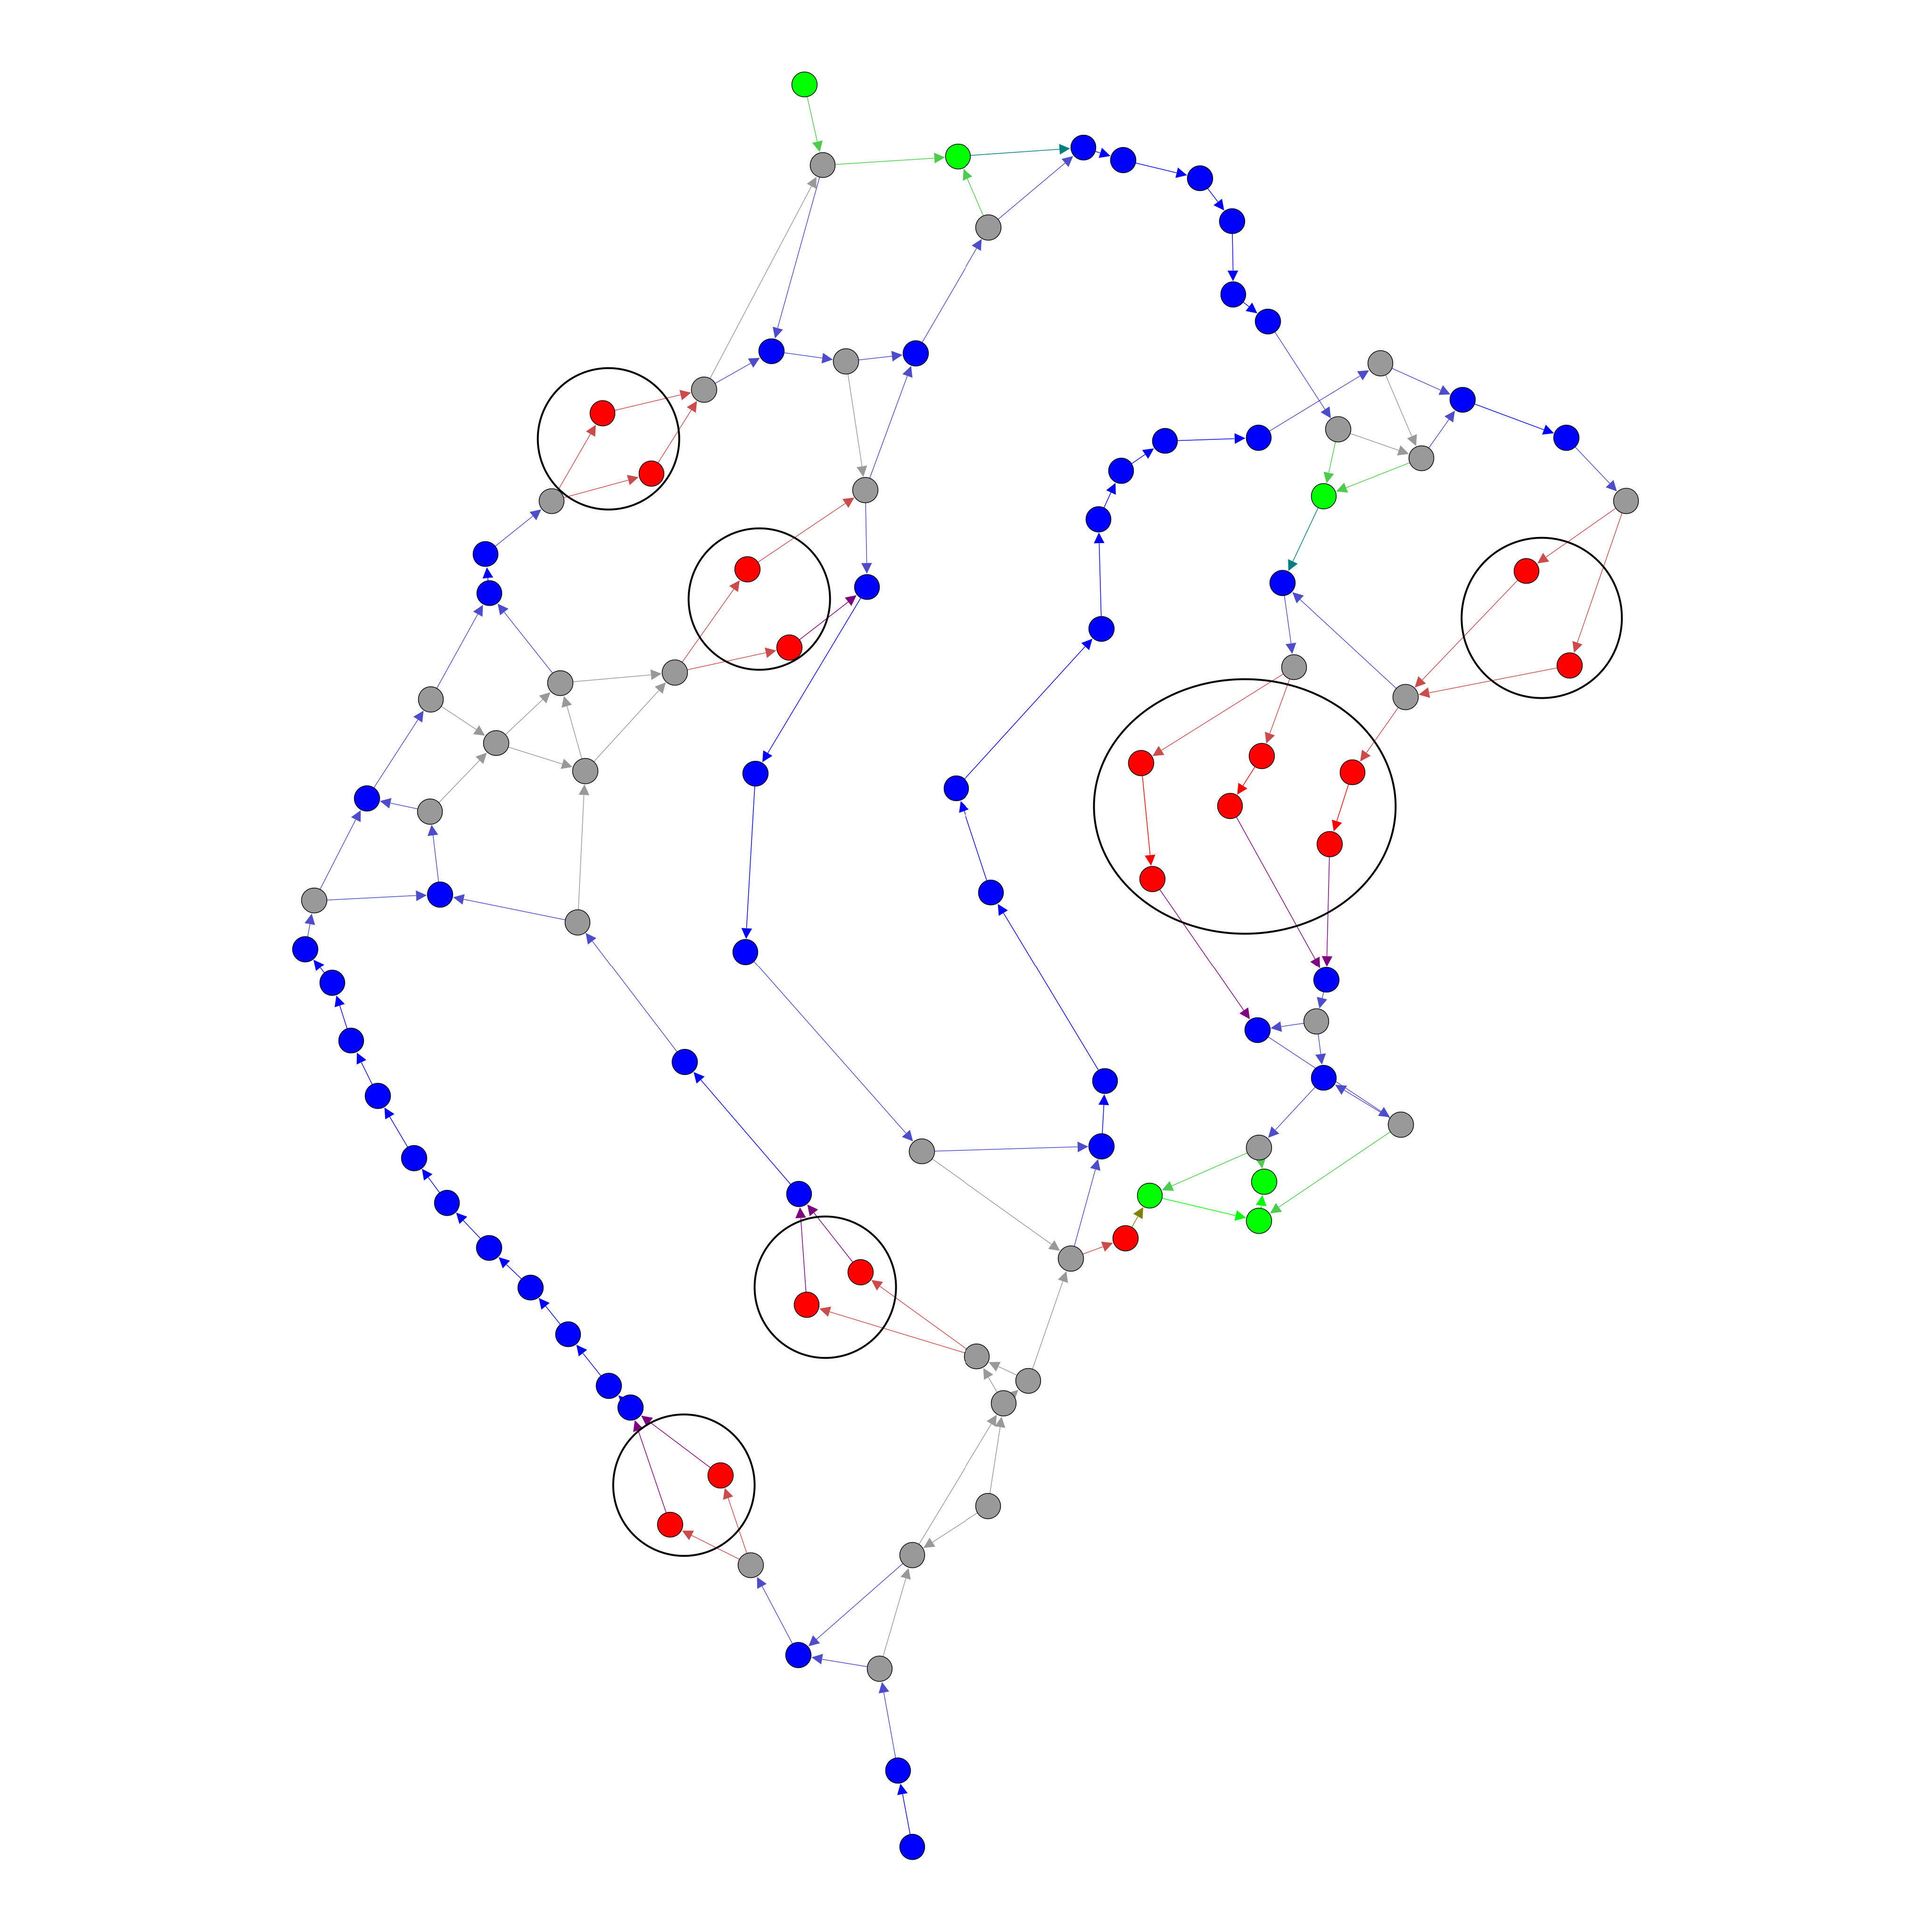
\includegraphics[scale=0.1]{experimentation/deadlock/deadlock.png}}
	\caption{Mixing of double-signed blocks(blue/grey) and half-signed blocks(red) in MultiChain.}
	\label{fig:deadlock-double}
\end{figure}

